\documentclass[a4paper, 10pt]{article}
\usepackage[utf8]{inputenc}
\usepackage{verbatim}
\usepackage{float}
\usepackage{listings}
\usepackage{graphicx}
\usepackage{a4wide}
\usepackage{color}
\usepackage{amsmath}
\usepackage{amssymb}
\usepackage[dvips]{epsfig}
\usepackage[toc,page]{appendix}
\usepackage[T1]{fontenc}
\usepackage{cite} % [2,3,4] --> [2--4]
\usepackage{shadow}
\usepackage{hyperref}
\usepackage{titling}
\usepackage{marvosym }
\usepackage{physics}

\usepackage{subcaption}
\usepackage[noabbrev]{cleveref}
\usepackage{wasysym}
\usepackage{changepage}


\renewcommand{\topfraction}{.85}
\renewcommand{\bottomfraction}{.7}
\renewcommand{\textfraction}{.15}
\renewcommand{\floatpagefraction}{.66}
\renewcommand{\dbltopfraction}{.66}
\renewcommand{\dblfloatpagefraction}{.66}
\setcounter{topnumber}{9}
\setcounter{bottomnumber}{9}
\setcounter{totalnumber}{20}
\setcounter{dbltopnumber}{9}


\setlength{\droptitle}{-10em}   % This is your set screw

\setcounter{tocdepth}{2}

\lstset{language=c++}
\lstset{alsolanguage=[90]Fortran}
\lstset{basicstyle=\small}
\lstset{backgroundcolor=\color{white}}
\lstset{frame=single}
\lstset{stringstyle=\ttfamily}
\lstset{keywordstyle=\color{red}\bfseries}
\lstset{commentstyle=\itshape\color{blue}}
\lstset{showspaces=false}
\lstset{showstringspaces=false}
\lstset{showtabs=false}
\lstset{breaklines}
\title{FYS3150/4150 - Project 2 \\
  Nummerical methods for solving Schröedinger equation for two different potentials}
\author{Aram Salihi$^1$, Adam Niewelgowski$^1$ \\
  \small $^1$Department of Physics, University of Oslo, N-0316 Oslo, Norway}
\begin{document}
\maketitle
\begin{abstract}
In this project we have solved Schröedinger equation for both interacting and non-
interacting case. The potential we choosed is the harmonic oscillator and the cloumb potential.
When increasing the angular frequency in the harmonic oscillator the harmonic oscillator well
is narrower and starts to dominate the coloumb potential. Thus showing that for large $\omega_{r}$
the interacting force becomes neglible. For this project we used the jacobi method and
armadillos eigenvalue solver. Comparing these two methods, we found out that armadillos solver is
more effiecient and easier to use.
\end{abstract}
\tableofcontents
\section{Introduction:} In this project we will be solving Schröedingers equation for two electrons for
two different cases: Non and interacting case. For this we will be using cloumb potential with the harmonic
oscillator potential well (interacting case), and harmonic oscillator alone (non-interacting). The motivation behind
this project is to show when the angular frequency in harmonic oscillator increases the coloumb potential becomes more and more neglible.
Due to the depth of the harmonic oscillator well is shrinked. Today such topic is highly active reasch field in solid state physics (semi-conductors, etc..) for different purposes.
Some of this purposes is presented in \cite{loss}.
\vspace{3mm}
\\
This problem can be turned into a eigenvalue problem and can be easily be solved by using different
types of nummerical methods. For this project we will be using jacobi's method and armadillos built-in function and benchmark
those two methods against each other.
\section{Theoretical Model:}
\subsection{Jacobi rotation:} Jacobi rotation or the so called Jacobis algorithm,
is a alogirthm which turns any given matrix $\mathbf{A}$ into a diagonal matrix $\mathbf{A_{D}}$.
This is done by multiplying a set of orthogonal transformation $\mathbf{J}_{i}$, $N$ times until
a diagonal matrix is formed. Thus each time $\mathbf{J}_{i}$ is multiplied an entry in
$\mathbf{A}$ is zeroed out.
\begin{align}
  \mathbf{A_{D}} = \mathbf{J}^{T}_{N}....\mathbf{J}^{T}_{1}\mathbf{A}
  \mathbf{J}_{1}....\mathbf{J}_{N}
\end{align}
A more detailed expalination is provided here \cite{morten2}.
Since $\mathbf{J}_{i}$ is a orthogonal transformation matrix it preserves the properties and
the eigenvalues of $\mathbf{A}$. Thus, this method is a outstanding method
to calculate the eigenvalues for a any given matrix due to its simplicity, but slow
compared to algorithms (this will be discussed in detailed later). Since $\mathbf{A}_{D}$
is a diagonal matrix the eigenvlaues is along the diagonal:
\begin{align}
\mathbf{A}_{D} =
\begin{pmatrix}
\lambda_{1} & ... & .... & 0 & ... & 0\\
0 & \lambda_{2} & ... & ... &... &. \\
. & . &\lambda_{3} & ... & ... & . \\
. & .. & . & \lambda_{4} & ... & . \\
. & ..  & ... & . &... & 0 \\
0 & .. & ... & ... & 0 & \lambda_{N} \\
\end{pmatrix}
\end{align}
Where $\lambda_{i}$ is the eigenvalues of matrix $\mathbf{A}$ and $\mathbf{A}_{D}$.
\subsubsection{Properties of orthogonal transformation:} We will now show that the
orthogonal transformation preserves the dot product and orthogonality. Consider
a orthonormal vector $\mathbf{v}$ and transformation matrix $\mathbf{J}$. This orthogonal
transformation matrix has the property:
\begin{align}
  \mathbf{J}^{T} = \mathbf{J}^{-1}
\end{align}
Notice that our orthonormal vectors form a basis $\mathcal{B} = \{\mathbf{v}\}$, thus
$v_{i}^{T}v_{j} = \delta_{ij}$, where $\delta_{ij}$ is the kronecker delta .
Further we will consider a vector $\mathbf{w} =\mathbf{J}\mathbf{v}$. The question is:
"What will happen if we take the dot product of $\mathbf{w}$ with itself?". Consider the following:
\begin{align}
  \mathbf{w}\cdot\mathbf{w} = w_{i}^{T}w_{j} = \left(\mathbf{J}v_{i}\right)^{T}\mathbf{J}v_{j}
  = v_{i}^{T}\mathbf{J}^{T}\mathbf{J}v_{j} =  v_{i}^{T}\mathbf{J}^{-1}\mathbf{J}v_{j} = v_{i}^{T}v_{j}
  = \delta_{ij}
\end{align}
Thus:
\begin{align}
  \mathbf{w}\cdot\mathbf{w} = w_{i}^{T}w_{j} = \delta_{ij}
\end{align}
\subsection{Schröedinger Equation:} As previously mentioned we will be solving the
three dimensional Schröedinger equation for harmonic oscillator and the coloumb potential:
\begin{align}
  V(r) = \frac{1}{2}m\omega^{2}\mathbf{r}^{2}
\end{align}
Where $\mathbf{r}$ is the position vector for center of mass for the electrons and
$\omega$ is the frequency. We are going to define the potential as following.
\begin{align}
  V(r) = \frac{1}{2}k\mathbf{r}^{2}
\end{align}
The constant $k$ defines the steepness of the well. The coloumb potential:
\begin{align}
  V(r) = \frac{q}{4\pi \epsilon_{0}r}
\end{align}
The time independent
Schröedinger equation is mathematically defined as:
\begin{align}
  \frac{\hbar^{2}}{2m}\nabla^{2}\Psi + V(r)\Psi = E\Psi
\end{align}
Since the potential is radially symmetric, the angular part can be dropped.
Thus:
\begin{align}
  -\frac{\hbar^{2}}{2m}\left(\frac{1}{r^{2}}\dv{r}r^{2}\dv{r} -
  \frac{l(l+1)}{r^{2}}\right)R(r) + V(r)R(r) = ER(r)
\end{align}
Where $l$ is the oribtal angular momentum and $E$ is the energy in the system.
Doing the following substituion $R(r) = u(r)/r$ (\cite{gg}) we can rewrite our equation to:
\begin{align}
  -\frac{\hbar^2}{2m}
  \frac{d^2}{dr^2}u(r)+\left(V(r)+
  \frac{l(l+1)}{r^2}\frac{\hbar^2}{2m}\right)u(r)=Eu(r)
\end{align}
We will now introduce a dimensionless distance variable $\rho = r/\alpha$ where
$\alpha$ has dimension length. After some algebra, the Schröedinger equation can then be formulated as
(in this project \cite{p2} we have choosen to set $l = 0$):
\begin{align}
  -\frac{d^2}{d\rho^2}u(\rho)+V(\rho)u(\rho)=\lambda u(\rho)
\end{align}
where $\lambda$ is the dimensionless energy eigenvalues defined as:
\begin{align}
  \lambda = \frac{2m\alpha^{2}}{\hbar^{2}}E
\end{align}
Note that:
\begin{align}
  \alpha^{4} = \frac{\hbar^{2}}{mk}
\end{align}
The potential will look like:
Non-interacting:
\begin{align}
  V_{HarmonicOscillator}(\rho) = \omega_{r}\rho^{2}
\end{align}
where $\omega_{r}$ is the characteristic frequency defined in (\cite{p2})
interacting:
\begin{align}
  V = V_{HarmonicOscillator}(\rho) +   V_{Coloumb}(\rho) = \omega_{r}\rho^{2} + 1/\rho
\end{align}
\subsection{Schröedinger's equation and the eigenvalue problem:}
Recall from previous the reformulation of Schröedingers equation:
\begin{align}
  -\frac{d^2}{d\rho^2}u(\rho)+V(\rho)u(\rho)=\lambda u(\rho)
\end{align}
This can be turned into a eigenvalue problem. We will now define a vector
$\mathbf{u}$, a square diagonal matrix $\mathbf{V}$ (with the potentials on its diagonal element).
The derivative operator can be written as toeplitz matrix $\mathbf{T}$ with $2/h^{2}$ on its main diagonal
and $-1/h^{2}$, where $h$ is the stepsize.
\begin{align}
  \label{matrix form}
\underbrace{\left(\mathbf{T} + \mathbf{V}\right)}_{\mathbf{A}}\mathbf{u}(\rho) = \lambda\mathbf{u}(\rho)
\end{align}
where we will define the main, upper and lower diagonal as:
\begin{align}
  d_{i} = \frac{2}{h^{2}} + V_{i} \qquad e_{i} = -\frac{1}{h^{2}}
\end{align}
Thus this can be discretized, and will have following look:
\begin{align}
  d_{i}u_{i} + e_{i-1}u_{i-1} + e_{i+1}u_{i+1} = \lambda u_{i}
\end{align}
\subsection{boundary conditions:} In this project we will be solving the
Schröedinger equation for Dirichlet boundaries. For $u_{0} = u_{N} = 0$ we have:
\begin{align}
(d_{1} - \lambda)u_{1} + e_{2}u_{1} = 0
\end{align}
\begin{align}
(e_{N-1} + e_{N+1})u_{1} = 0
\end{align}
This means we can remove these values the rows and coloumns and simply add zero
on the top and bottom on the eigenvector.

\section{Method}
\subsection{Algorithm}
To study different situations of electrons in a harmonic oscillator potential,
we had to develope Jacobi method algorithm (which is heavily inspired by the code found in
\cite{morten2}). The pseudo code of the
transformations is (see github repository for all the source codes implemented
with c++)
\begin{lstlisting}
	while(biggest_of_diagonal < eps AND iterations < max_iterations)
         JacobiRotation(A, k, l)
         FindMaxOffDiagonal(A, k, l)
\end{lstlisting}

The idea behind this algorithm is to perform the rotation on the biggest off
diagonal element in the matrix A, which has index \(k\) and \(l\). After every
rotation, we are updating the indexes with \textit{FindMaxOffDiagonal}.
Diagonalization is done when the biggest off diagonal element is smaller than
given \textit{eps}, which is an approximation to  zero.

\subsection{Unit tests}
We applied both of the functions shown in the pseudo code on a
small test matrices, to ensure that our algorithm is working the way we want it
to before we moved on the bigger matrices to solve quantum problems.
First, we checked the \textit{FindMaxOffDiagonal} by simply checking if it
returned the correct value
\begin{lstlisting}
	find_max_offdiag(A,k,l,n);

    if((abs((A(l,k))-(abs(biggest_element))) < eps) && (k == 2) && (l == 1)){
        //PASSED
    }
    else{
        cout << "Finding max offdiag element test FAILED - need to check the find_max_offdiag function" << endl;
        exit(1);
    }
\end{lstlisting}

where \textit{biggest\_element} is the biggest value placed on the off-diagonal
in the test matrix.

To test the \textit{JacobiRotation} we had to implement the whole algorithm
(together with \textit{FindMaxOffDiagonal} as shown in pseudo code above) to be able to check

\begin{enumerate}
\item eigenvalues produced by code against the analytical eigenvalues
\item orthogonality of the eigenvectors produced
\item symmetry conversation of a test matrix
\end{enumerate}

\subsection{Parameters}
After passing all of the tests, we were ready to solve quantum problems. We
were interested in two scenarios, one and  two electrons in a potential well.
With only one electron we had harmonic oscillator potential. With two electrons
we had to add the Coulomb repulsive force between the particles. We were
interested to study how the eigenfunction will behave with different
\(\omega_{r}\) in range between \(0.01\) to \(5.0\).

In addition we needed to find a good nummerical fit to approximate \(\rho_{max}=\infty\) to match
a given range of \(\omega_{r}\). We chose \(\rho_{max} = 40\) for \(\omega_{r}
= 0.01\) and \(\rho_{max}= 5\) for \(\omega_{r} = \{0.5, 1.0, 5.0\}\).
\section{Results}

\subsection{Efficiency}
As we can see in section 3.1, Jacobi
transformation algorithm does operate under two main conditions in the
\textit{while} loop, either the
maximum off-diagonal element will be approximately zero or we exceed given
transformation limit.  Diagonalization of our matrix, depends on the matrix
itself and it's dimensionality. The graph below shows number of rotations
needed to diagonalize matrices with different dimensions.
\begin{figure}[h!]
  \centering
  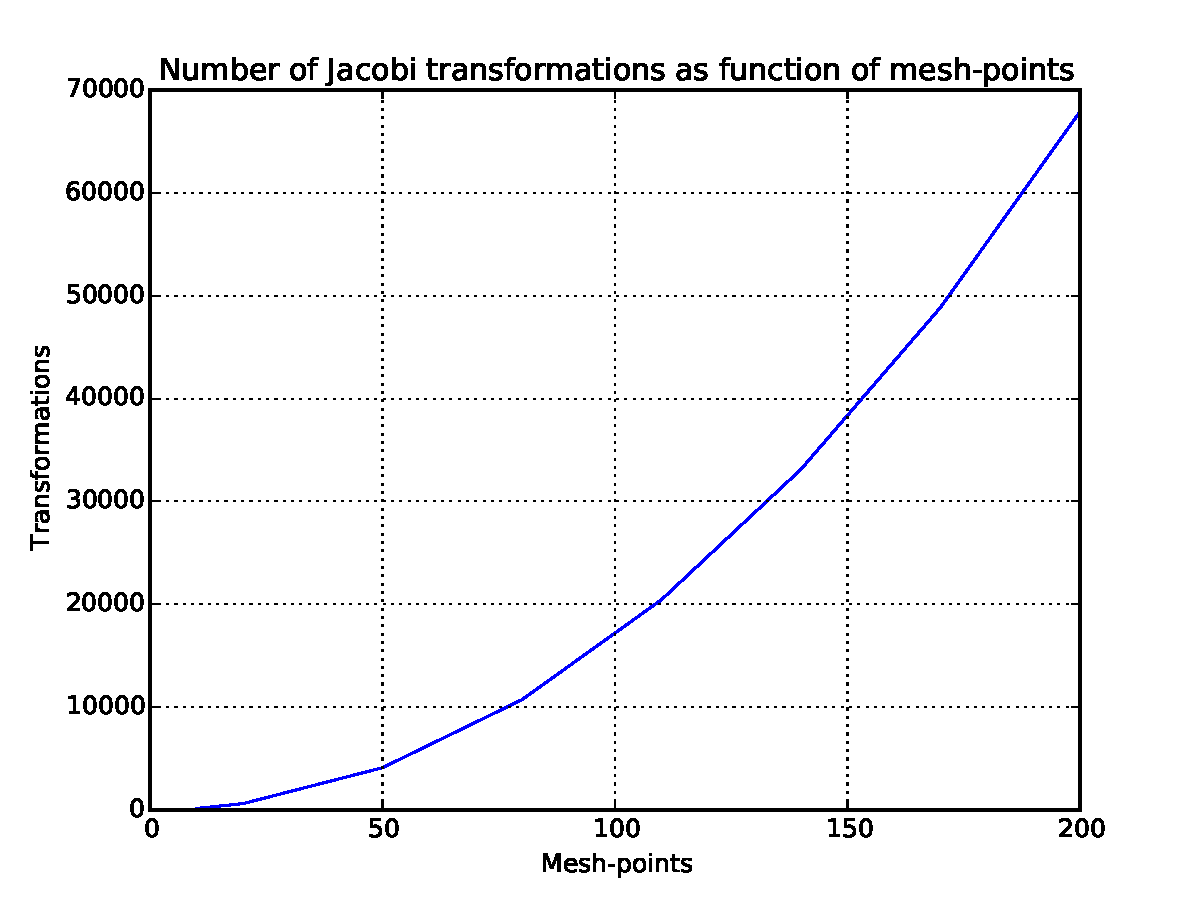
\includegraphics[width=8cm]{transformations.pdf}
  \caption{}
\end{figure}

The time consumption compared with in-build armadillo function to find
eigenpairs is significant.

% tabell med tidene - sendte den i en av tex filene, finner den ikke her

%og

% plotTime
\begin{figure}[h!]
  \centering
  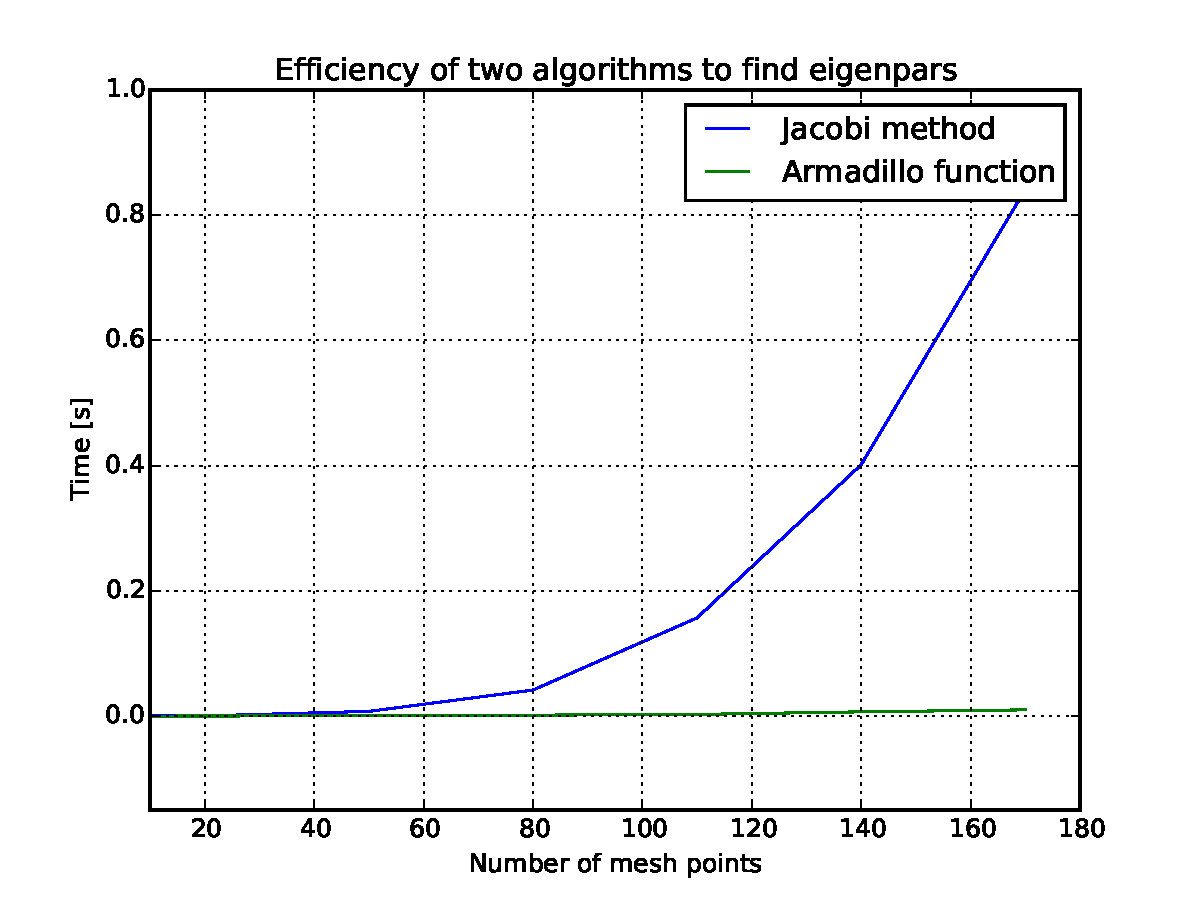
\includegraphics[width=8cm]{timePlot.pdf}
  \caption{}
\end{figure}
\subsection{Ground state eigenfunctions}

%present our results from plotting eigenfunctions with different potentials (4 figurer)


\begin{figure}[H]
        \centering
        \begin{subfigure}[b]{0.42\textwidth}
            \centering
            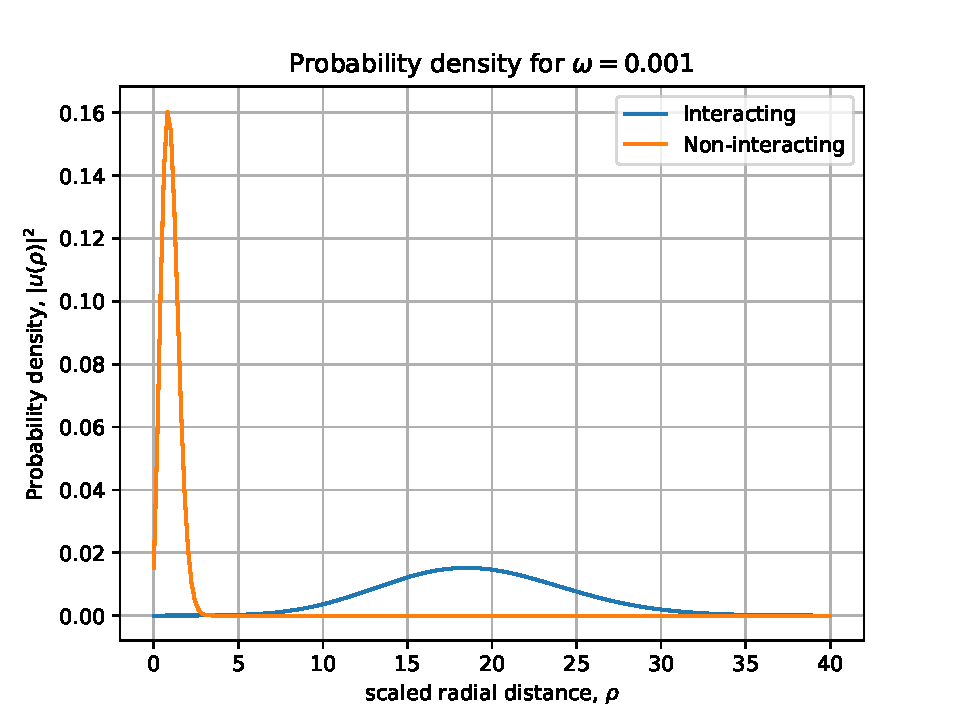
\includegraphics[width=\textwidth]{Probability_density_w001.pdf}
            \caption{$\omega_{r} = 0.01$}
        \end{subfigure}
        \hfill
        \begin{subfigure}[b]{0.42\textwidth}
            \centering
            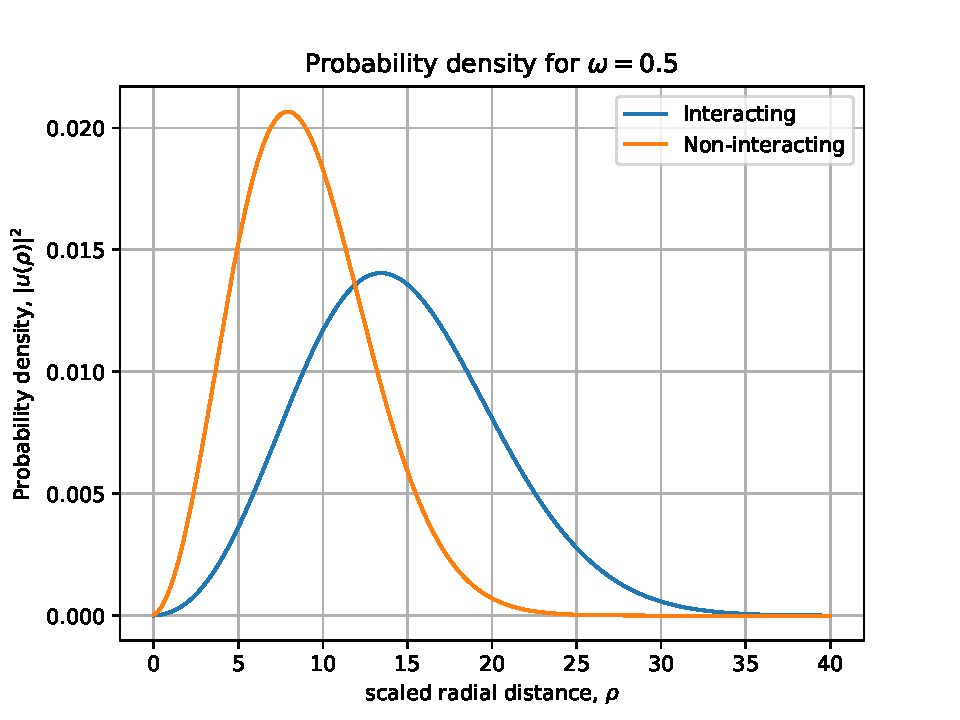
\includegraphics[width=\textwidth]{Probability_density_w05.pdf}
            \caption{$\omega_{r} = 0.5$}%
        \end{subfigure}
        \vskip\baselineskip
        \begin{subfigure}[b]{0.42\textwidth}
            \centering
            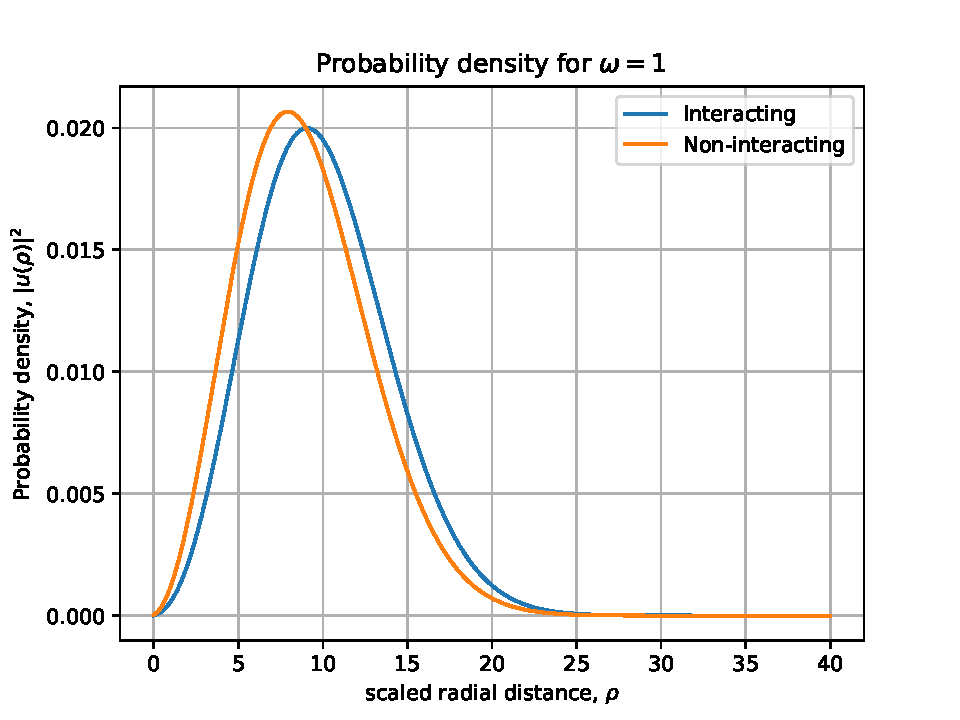
\includegraphics[width=\textwidth]{Probability_density_w1.pdf}
            \caption{$\omega_{r} = 1$}%
        \end{subfigure}
        \quad
        \begin{subfigure}[b]{0.42\textwidth}
            \centering
            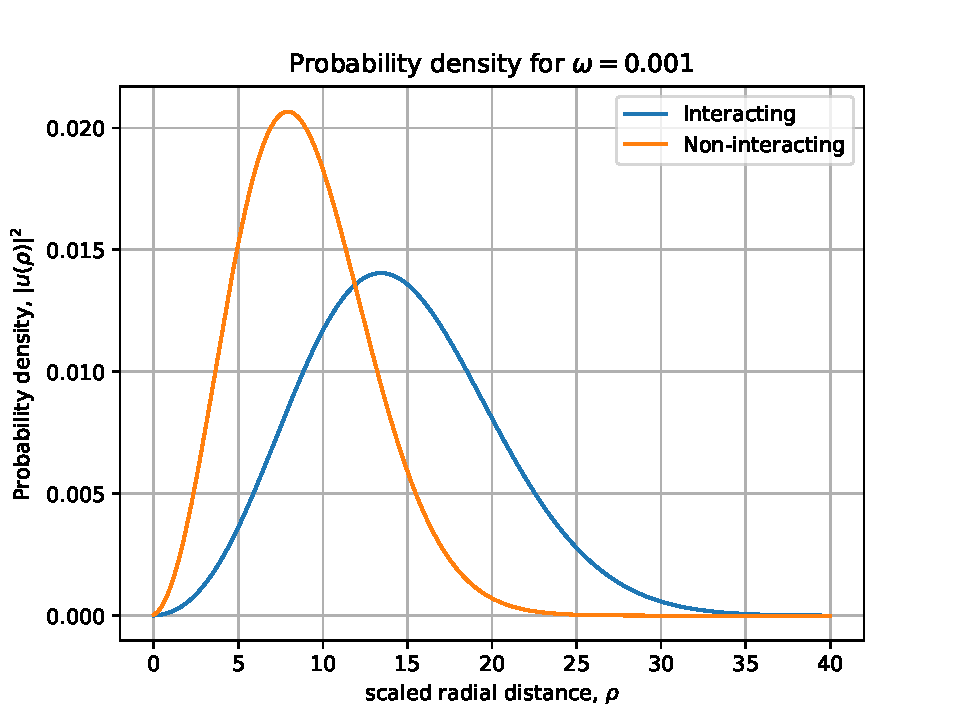
\includegraphics[width=\textwidth]{Probability_density_w5.pdf}
            \caption{$\omega_{r} = 5$}%
        \end{subfigure}
        \caption{This following four plots shows how the probability density of the ground
        state eigenfunction varies, when tweaking the frequency $\omega_{r}$. Here we have
        squared the groundstate eigenfunction and plotted against the gridpoints used.}
        \label{dd}
    \end{figure}
    \newpage
\section{Discussion}
\subsection{Efficiency}
Diagonalization of a given matrix using Jacobi method depends on the matrix
itself. Even if we set the limit of transformations to be infinity, some of the
matrices does not converge to diagonal matrix, because off-diagonal elements
never become zero or close to zero. This can happen in cases where off-diagonal
elements which are already close to zero after a few transformations, become
non-zero again after next transformation which aims to zero out a different
off-diagonal element. In these cases we will never get a diagonalized matrix.

Armadillo in-build function to solve eigenproblems is optimalized and runs very
quickly even if dimension of a matrix increases. This is why we used armadillo
to get our eigenvectors which we used to plot ground state eigenfunctions.
Second reason is that armadillo gives sorted output pairs of eigenvalues and
eigenvectors. If we would like to use Jacobi method to plot ground state
eigenfunction, we would have to use few more FLOPS and iterations to find the
row index of absoulte value of the smalles smallest diagonal element
(eigenvalue). This index corresponds to the column index in eigenvector matrix.

\subsection{Groundstate eigenfunctions} As expected when increasing the frequency of
the harmonic oscillator the gap between the electrons are narrower. For the interacting
case we see that when this parameter $\omega_{r}$ is increased, the harmonic potential
dominates the coloumb potential. In graph (d) in (\ref{dd}) we see that this is not true,
but it should be almost overlap of those two graphs, but this is due to some error when some files are
produced. Thus when increasing $\omega_{r}$ the harmonic potential becomes more and more
dominant in the interacting case. This can be seen when equating the coloumb potential and
harmonic oscillator. The relation between the distance and frequency is given by:
\begin{align}
  \rho < \omega_{r}^{-1/3}
\end{align}
For the non interacting case we see that the
width of the potential becomes narrower thus the electrons oscillator closer relative to each other. The eigenfunctions and its corresponding
eigenvalue was found by using c++ library armadillo, due its efficiency (compared to jacobis method which is significantly slower )
and sorting the eigenfunctions with is correspongding eigenvalue.
\section{Conclusion} In this project we solved Schröedingers equation for two different
potentials. As it turns out for the interacting case when presenting the coloumb potential.
The electrons gets closer as we increase the frequency $\omega_{r}$, this is because
the coloumb potenial is dominated by the harmonic potential. By using intuition this make sense
since the gap in the harmonic potential is getting narrower.
\vspace{3mm}
\\
For the nummerical part: The jacobi method we used was nummerically stable but slow and tedious compared to
armadillos matrix equation solver. Note that (as mentioned previously) the groundstate eigenfunctions
were found by using armadillo, this is due to efficiency and that armadillo sorts eigenfunction with its
correspong eigenvalue.
\subsection{For future work}
\begin{itemize}
  \item we can look deeper into our code and find why the last plot
  in the probability density is not overlaping
  \item comparing the nummerical solution and analytical solution found in \cite{taut}
\end{itemize}

\newpage
\bibliographystyle{apalike}
\bibliography{project2}
\end{document}
